%Dokumentklasse

%draft als optionohne bilder für bessere performance
%\documentclass[a4paper,12pt,draft]{scrreprt}

%normal mit Bildern
\documentclass[a4paper,12pt]{scrreprt}

\usepackage[left= 3cm,right = 3cm, bottom = 3cm,top = 3cm]{geometry}
%\usepackage[onehalfspacing]{setspace}

% ============= Packages =============

% Dokumentinformationen
\usepackage[
pdftitle={Praktikum - Umwelttechnik},
pdfsubject={},
pdfauthor={Roman-Luca Zank},
pdfkeywords={},	
%Links nicht einrahmen
hidelinks
]{hyperref}

%nur Text zum prüfen des Umfangs

% Standard Packages
%\usepackage[bottom]{footmisc}
\usepackage[utf8]{inputenc}
\usepackage[ngerman]{babel}
\usepackage[T1]{fontenc}

%\usepackage{helvet}
%\renewcommand{\familydefault}{\sfdefault}

\usepackage{graphicx}
\graphicspath{{img/}}
\usepackage{mhchem}
\usepackage{fancyhdr}
\usepackage{lmodern}
\usepackage{color}
\usepackage{placeins}
\usepackage{booktabs}
\usepackage{caption}
\usepackage[list=true]{subcaption}
\usepackage{longtable}
\usepackage{tikz}
\usepackage{lastpage}
\usepackage{pgfplots}
%Abb. statt Abbildung
\addto\captionsngerman{%
	\renewcommand{\figurename}{Abb.}%
	\renewcommand{\tablename}{Tab.}%
}


%Einheitenpackage
\usepackage{siunitx}  
\sisetup{	locale = DE, 
	per-mode=fraction,
	inter-unit-product=\ensuremath{\cdot},
	detect-weight = true,
	quotient-mode=fraction
}
%neue Einheiten definieren
\DeclareSIUnit\xyz{xyz}		
\DeclareSIUnit{\mpercent}{Ma\%}

%Automatisch cdot statt *
\DeclareMathSymbol{*}{\mathbin}{symbols}{"01}



%\setcounter{lofdepth}{2}      %für subfigures in list of figures

%Tabelle
\usepackage{tabularx}
\usepackage{tabulary}

%%Verzeichnispackages
%\usepackage{natbib}

%\usepackage{hyperref}
%\newcites{

% zusätzliche Schriftzeichen der American Mathematical Society
\usepackage{amsfonts}
\usepackage{amsmath}

%Abkürzungsverzeichnis
\usepackage{acronym}

%kein Abstand bei neuem Kapitel vom Seitenanfang
%\vspace*{2.3\baselineskip} = ORIGINAL
\renewcommand*{\chapterheadstartvskip}{\vspace*{.0\baselineskip}}

%nicht einrücken nach Absatz
\setlength{\parindent}{0pt}


\urlstyle{same}

% ============= Kopf- und Fußzeile =============
\pagestyle{fancy}
%
\lhead{}
\chead{}
\rhead{}%\slshape }%\leftmark}
%%
\lfoot{}
\cfoot{}
\rfoot[{\thepage\ of \pageref*{LastPage}}]{Seite \thepage\ von \pageref*{LastPage}}
%%
\renewcommand{\headrulewidth}{0pt}
\renewcommand{\footrulewidth}{0pt}
\renewcommand{\chapterpagestyle}{fancy}

%Fußnotelinie
%\let\footnoterule

%Fußnote mit Klammer
\renewcommand*{\thefootnote}{(\arabic{footnote})}

% ============= Package Einstellungen & Sonstiges ============= 
%Besondere Trennungen
%\hyphenation{De-zi-mal-tren-nung}
\usepackage[none]{hyphenat}
\hyphenpenalty=5000
\tolerance=5000
\providecommand\phantomsection{}

\usepackage{mathtools}

\usepackage{yfonts}
\usepackage[T1]{fontenc}
%!!!!!!!!!!!!!!!!!!!!!!!!!!!!!!!!!!!
%\usepackage[T1]{fontenc}
%\usepackage{yfonts}
%\input MorrisIn.fd
%\newcommand*\initfamily{\usefont{U}{MorrisIn}{xl}{n}}
%!!!!!!!!!!!!!!!!!!!!!!!!!!!!!!!!!!!

% ============= Dokumentbeginn =============

\begin{document}
%!!!!!!!!!!!!!!!!!!!!!!!!!!!!!!!!!!!!!!!!!!
%\normalfont\swabfamily
%\normalfont\gothfamily
%!!!!!!!!!!!!!!!!!!!!!!!!!!!!!!!!!!!!!!!!!!!!

%Seiten ohne Kopf- und Fußzeile sowie Seitenzahl
\pagestyle{empty}

%\begin{center}
\begin{tabular}{p{\textwidth}}


\begin{center}

\includegraphics[scale=0.75]{logos.jpg}\\
\end{center}


\\

\begin{center}
\LARGE{\textsc{
Protokoll \\
Umwelttechnik\\
}}
\end{center}

\\

%\begin{center}
%\large{Fakultät für Muster und Beispiele \\
%der Hochschule Musterhausen \\}
%\end{center}
%
%\\

\begin{center}
\textbf{\Large{V1 - Thermische Abfallbehandlung}}
\end{center}

\begin{center}
	\large{Gruppe 1.2 (BCUT3)}
\end{center}


\\
%\begin{center}
%zur Erlangung des akademischen Grades\\
%Bachelor of Engineering
%\end{center}


%\begin{center}
%vorgelegt von
%\end{center}

\begin{center}
\Large{\textbf{Teilnehmer:}} \\ 
\end{center}
\begin{center}
\large{	Christoph Hecht \\
Willy Messerschmidt \\
Roman-Luca Zank\\}
\end{center}


\\

\begin{center}
\begin{tabular}{lll}
\large{\textbf{Protokollführer:}} & & \large{Roman oder Willy} \\
& & email@stud.hs-merseburg.de\\
&&\\
\large{\textbf{Datum der Versuchsdurchführung:}}&& \large{05.11.2019 \& 19.11.2019}\\
&&\\
\large{\textbf{Abgabedatum:}}&& \large{00.00.2019}
\end{tabular}
\end{center}

\\ \\ \\ \\ \\ \\
\large{Merseburg den \today}

\end{tabular}
\end{center}


%\include{14_danksagungen}

%\include{15_zusammenfassung}

% Beendet eine Seite und erzwingt auf den nachfolgenden Seiten die Ausgabe aller Gleitobjekte (z.B. Abbildungen), die bislang definiert, aber noch nicht ausgegeben wurden. Dieser Befehl fügt, falls nötig, eine leere Seite ein, sodaß die nächste Seite nach den Gleitobjekten eine ungerade Seitennummer hat. 
\cleardoubleoddpage

% Pagestyle für Titelblatt leer
\pagestyle{empty}

%Seite zählen ab
\setcounter{page}{0}

%Titelblatt
\begin{center}
\begin{tabular}{p{\textwidth}}


\begin{center}

\includegraphics[scale=0.75]{logos.jpg}\\
\end{center}


\\

\begin{center}
\LARGE{\textsc{
Protokoll \\
Umwelttechnik\\
}}
\end{center}

\\

%\begin{center}
%\large{Fakultät für Muster und Beispiele \\
%der Hochschule Musterhausen \\}
%\end{center}
%
%\\

\begin{center}
\textbf{\Large{V1 - Thermische Abfallbehandlung}}
\end{center}

\begin{center}
	\large{Gruppe 1.2 (BCUT3)}
\end{center}


\\
%\begin{center}
%zur Erlangung des akademischen Grades\\
%Bachelor of Engineering
%\end{center}


%\begin{center}
%vorgelegt von
%\end{center}

\begin{center}
\Large{\textbf{Teilnehmer:}} \\ 
\end{center}
\begin{center}
\large{	Christoph Hecht \\
Willy Messerschmidt \\
Roman-Luca Zank\\}
\end{center}


\\

\begin{center}
\begin{tabular}{lll}
\large{\textbf{Protokollführer:}} & & \large{Roman oder Willy} \\
& & email@stud.hs-merseburg.de\\
&&\\
\large{\textbf{Datum der Versuchsdurchführung:}}&& \large{05.11.2019 \& 19.11.2019}\\
&&\\
\large{\textbf{Abgabedatum:}}&& \large{00.00.2019}
\end{tabular}
\end{center}

\\ \\ \\ \\ \\ \\
\large{Merseburg den \today}

\end{tabular}
\end{center}
 %Prokolle
%\begin{center}
\begin{tabular}{p{\textwidth}}


\begin{center}

\includegraphics[scale=0.75]{img/logos.jpg}\\
\end{center}


\\

\begin{center}
\LARGE{\textsc{
Recherche \\
Rückgewinnung von Ammoniak aus Industrieabwässern\\
}}
\end{center}

%\begin{center}
%\large{Fakultät für Muster und Beispiele \\
%der Hochschule Musterhausen \\}
%\end{center}
%
%\\
 \\
 
\begin{center}
\textbf{\Large{Seminararbeit in Medienrecherche}}
\end{center}

\begin{center}
	\large{im WiSe 2019}
\end{center}
 \\
%\begin{center}
%zur Erlangung des akademischen Grades\\
%Bachelor of Engineering
%\end{center}


\begin{center}
\large{vorgelegt von}
\end{center}
\\


\begin{center}
\Large{\textbf{Roman-Luca Zank}} \\
\end{center}

\begin{center}
3. Semester \\
Chemie- und Umwelttechnik \\
\end{center}


\begin{center}
\begin{tabular}{lll}
	\textbf{E-Mail:} & & romanzank@mail.de\\
	\textbf{Matrikelnummer:} & &25240\\
	\textbf{Adresse:} & &Platz der Bausoldaten 2, Zimmer 224\\
	\textbf{Ort:} & &06217 Merseburg\\
	&& \\
	\textbf{Prüfer:} & & Dr. Frank  Baumann\\
\end{tabular}
\end{center}

\\ \\ \\ \\ \\
\large{Merseburg, \today}

\end{tabular}
\end{center}
 %Seminar-/Abschlussarbeit

% Pagestyle für Rest des Dokuments
\pagestyle{fancy}

%Inhaltsverzeichnis
\tableofcontents

%Inhalt
%%Verzeichnis aller Bilder
\label{sec:bilder}
\listoffigures
\addcontentsline{toc}{chapter}{Abbildungsverzeichnis}
\thispagestyle{empty}

%Verzeichnis aller Tabellen
\label{sec:tabellen}
\listoftables
\addcontentsline{toc}{chapter}{Tabellenverzeichnis}
\thispagestyle{empty}

%Abkürzungsverzeichnis
%\setlength{\columnsep}{20pt}
%\twocolumn
%\addchap{Nomenklatur (fett)}
%\label{sec:abkurzung}
%\begin{acronym}
%	\acro{vbr} [\boldmath{$\dot{V}_{Br}$}] {Volumenstrom Brennstoff \\ (Erdgas)}
%	\acro{vml} [\boldmath{$\dot{V}_{L}$}] {Volumenstrom der Luft}
%	\acro{vwa} [\boldmath{$\dot{V}_{W\omega}$}] {Ausgangsvolumenstrom Wasser}
%	\\
%	\acro{mbr} [\boldmath{$\dot{m}_{Br}$}] {Massestrom Brennstoff \\ (Erdgas)}
%	\acro{ml}  [\boldmath{$\dot{m}_{L}$}] {Massenstrom Luft}
%	\acro{ma}  [\boldmath{$\dot{m}_{A}$}] {Massenstrom Abgas}
%	\acro{mwa} [\boldmath{$\dot{m}_{W\alpha}$}] {Eingangsmassenstrom Wasser}
%	\acro{mww} [\boldmath{$\dot{m}_{W\omega}$}] {Ausgangsmassenstrom Wasser}
%	\\
%	\acro{qbr} [\boldmath{$\dot{Q}_{Br}$}] {Wärmestrom Brennstoff \\ (Erdgas)}
%	\acro{qa}  [\boldmath{$\dot{Q}_{A}$}] {Wärmestrom Abgase}
%	\acro{qstr}[\boldmath{$\dot{Q}_{Str}$}] {Strahlungswärme}
%	\acro{qw}  [\boldmath{$\dot{Q}_{W}$}] {result. Wärmestrom Wasser}
%	\acro{qwe} [\boldmath{$\dot{Q}_{Weitere}$}] {Weitere Wärmeverluste}
%	\\
%	\acro{nbro} [\boldmath{$\dot{n}_{Br}$}] {Molstrom Brennstoff}
%	\acro{no2o} [\boldmath{$\dot{n}_{O_{2}}$}] {Molstrom Sauerstoff}
%	\\
%	\acro{wirkungE} [\boldmath{$\eta_{E}$}] {energetischer Wirkungsgrad}
%	\acro{wirkungF} [\boldmath{$\eta_{F}$}] {feuerungstechnischer\\ Wirkungsgrad}
%	\\
%	\acro{vT} [\boldmath{$\tau_{Vor}$}] {Heizvorlauftemperatur}
%	\acro{rT} [\boldmath{$\tau_{Rück}$}] {Heizrücklauftemperatur}
%	\acro{AT} [\boldmath{$\tau_{A}$}] {Abgastemperatur}
%	\acro{averlust} [\boldmath{$qA$}] {Abgasverlust}
%	\acro{co2}[\boldmath{$\%CO_{2}$}] {CO$_{2}$-Gehalt im Abgas}
%	\acro{o2} [\boldmath{$\%O_{2}$}] {O$_{2}$-Restgehalt im Abgas}
%	\\
%	\acro{heizbr} [\boldmath{$H_u$}$= 10,4 \frac{kWh}{m^3}$] {Heizwert \\ des Brennstoffes (Erdgas)}
%	\acro{dbr}[\boldmath{$\rho_{E}$}$= 0,7\frac{kg}{m^3}$] {Dichte \\ des Brennstoffes (Erdgas)}
%	\acro{dw} [\boldmath{$\rho_{W}$}$= 988\frac{kg}{m^3}$] {Dichte \\ des Heizfluides (Wasser)}
%	\acro{dl} [\boldmath{$\rho_{L}$}$= 1,2\frac{kg}{l}$] {Dichte der Luft}
%	\acro{cp} [\boldmath{$c_{pW}$}$= 4,1\frac{kJ}{kg*K}$] {spezifische \\ Wärmekapazität des Heizfluides (Wasser)}
%	\acro{nbr} [\boldmath{$M_{Br}= 16\frac{g}{mol}$}] {Molare Masse \\ des Brennstoffs}
%\end{acronym}
%\subsubsection{Aufrufen einer Abkürzung}
%\acs{rT}
%\begin{verbatim}
%\acs{Abkürzung}
%\end{verbatim}

%\onecolumn

\chapter{Aufgabenstellung}
\label{sec:aufgabenstellung}
%In der Aufgabenstellung wird (in eigenen Worten und ganzen Sätzen) formuliert, was das Ziel des 
%Versuches ist.  
%[Beachten Sie die eigentliche Aufgabenstellung in den Versuchsanleitungen sowie die Hinweise zur Auswertung!] 
Im Versuch 1 "`Thermische Abfallbehandlung"' wird eine der vorliegenden Abfallproben gewählt und nach Asche-, Chlor- und insbesondere Kohlenstoffgehalt charakterisiert. \\ \\
Der gesamte Versuch teilt sich dabei in zwei Versuchsteile. Im ersten Versuchsteil erfolgt die Kalibrierung des TIC-Moduls und die Bestimmung des Carbonatgehaltes in der Probe. Im zweiten Versuchsteil wird dann über Totalverbrennung in einer Brennkammer der thermisch vollständig zersetzte Abfall bilanziert.\\ \\
Besonders im Fokus steht in diesem Versuch die Plausibilität der Messwerte mit deren Interpreation, sowie die Fehleranfälligkeit mit Vor- und Nachteilen der einzelnen Messmethoden.


\chapter{Geräte und Chemikalien}
\label{sec:geraete}

\textbf{Geräte:}
\begin{itemize}
	\item TIC-Modul
	\item $CO_2$-Detektor
	\item PC mit Detektorsoftware
	\item Magnetrührer mit Heizplatte
	\item Analysewaage
	\item Trockenschrank
	\item Brennkammer (EA4000 Analytik Jena AG)
	\item Erlenmeyerkolben (min. \SI{50}{\milli \liter}, Schliff NS/29)
	\item Keramiktiegel (\SI{25}{\milli \liter} und \SI{50}{\milli \liter})
	\item Löffelspatel
\end{itemize}

\vspace*{5mm}

\textbf{Proben/Chemikalien:}
\begin{itemize}
	\item Müllprobe: Müll I
	\item destilliertes Wasser
	\item Schlifffett
	\item 30-40\%ige Phosphorsäure
	\item Natronlauge ($c_{NaOH}=\SI{11}{\mole \per \liter}$)
\end{itemize}




\chapter{Durchführung}
\label{sec:durchfuerung}
%Die Durchführung sollte so geschrieben sein, dass alle notwendigen Angaben für den folgenden Ergebnisteil enthalten sind. Das beinhaltet z.B. Volumina von filtrierten Flüssigkeiten und die Angabe von Verdünnungen. Mit der Beschreibung der Durchführung sollte der Versuch nachvollziehbar und wiederholbar sein. Bei einer sehr umfänglichen Versuchsbeschreibung kann auf die Praktikumsanweisung verwiesen werden (1). Die groben Schritte sollten trotzdem hier in eigenen Worten beschrieben werden. Falls sinnvoll, kann auch eine Abbildung des Versuchsaufbaus eingefügt werden (Abb. 1). 

Der Versuch 1 teilt sich in zwei Versuchsabschnitte bei denen eine Müllprobe anhand von Chlor-, Asche- und Kohlenstoffgehalt charakterisiert wird. \\
In diesem Versuch wurde "`Müll I"' als Abfallprobe gewählt.\\ 

%Versuchaufbau für Versuchsabschnitt 1
Der erste Versuchsteil erfolgt am Arbeitsplatz des TIC-Moduls. Er beschäftigt sich lediglich mit der Kalibrierung des TIC-Moduls, sowie der Bestimmung des Carbonatgehaltes in der jeweiligen Müllprobe.\\

%Durchführung
%Versuchsabschnitt 1
In diesem Versuchsabschnitt wird ca. $\SI{1}{\gram}$ der Müllprobe im Erlenmeyerkolben abgewogen. Da die Probe "`Müll I"' sehr grobes und trockenes Material enthält, wird das Substrat mit destilliertem Wasser benetzt, um eine bessere Durchmischbarkeit der Probe zu bewirken. Infolgedessen wird der Rührfisch zugegeben und die Innenseite des Erlenmeyerkolbenschliffes mit etwas Schlifffett versehen. Ist dies erfolgt, so kann der Erlenmeyerkolben in das TIC-Modul eingespannt werden. Der Kolben steht dann auf einer auf \SI{80}{\degreeCelsius} vorgewärmten Rührheizplatte. Das Schlifffett sollte an diesem Punkt ein entweichen des zugeführten Trägergases verhindern. Trägergas ist in diesem Versuch Sauerstoff, welcher einen konstanten Trägerfluss von \SI{16}{\liter \per \hour} einzuhalten hat. Spätestens an diesem Punkt werden der mit dem Computer verbundene \ce{CO2}-Detektor und Rührer eingeschaltet.\\
Nach diesen Vorbereitungen kann die Messung mittels \ce{CO2}-Detektor über die Software am Computer gestartet werden. Es wird dabei den Anweisungen der Software Folge geleistet. Nach die Basislinie vom Programm gefunden wurde, wird die Säure zum Austreiben des \ce{CO2} aus den Carbonaten zugesetzt. Dies erfolgt mit einer Hand-Dosier-Pumpe, welche über ein zwischengeschaltetes Ventil und einem Schlauch mit dem Erlenmeyerkolben und dem Phosphorsäurebehälter verbunden ist. Nach der Dosierung von zwei mal $\SI{5}{\milli \liter}$ Säure, wird das zum Erlenmeyerkolben geöffnete Ventil sofort wieder geschlossen. Ab diesem Punkt wird nun gewartet bis die Software ihre Messung beendet und die Fläche unter dem erzeugen Graphen integriert hat. Start- und Endpunkt der Integration müssen möglicherweise manuell korrigiert werden.\\
Diese Vorgehensweise bleibt für jegliche Müll- und Carbonatproben gleich. Mit den erzeugten Ergebnissen können dann Rückschlüsse auf den TIC-Gehalt in den jeweiligen Müllproben gezogen werden.
In diesem Fall erfolgte lediglich eine Zweifachbestimmung der reinen Carbonatproben. Bereits der zweite Messwert lag nah genug am gemessenen Wert der Abfallprobe.\\ 
Im Nachhinein wird die verbliebene Phosphorsäure in der TIC-Abfallprobe mittels $\SI{15}{\milli \liter}$ Natronlauge neutralisiert.
% Die Probe wird dann gewogen. Zur späteren Verwendung werden zu diesem Zeitpunkt ca. $\SI{3}{\gram}$ der originalen Abfallprobe in einen Keramiktiegel eingewogen. Zuletzt werden bis zum zweiten Praktikumstermin beide Proben innerhalb eines Keramiktiegels in den Trockenschrank  gestellt.

Dem folgend wird das Leergewicht zweier Keramiktiegel bestimmt.
Die zuvor analysierte Abfallprobe wird mitsamt der der Flüssigkeit in einen der beiden Keramiktiegel umgefüllt.  
In den anderen Tiegel werden ca. $\SI{3}{\gram}$ der originalen Abfallprobe eingewogen. Beide Tiegel werden beschriftet und anschließend für 14 Tage in den Trockenschrank gestellt.
\newpage
%Versuchsabschnitt 2

Der zweite Versuchsteil beginnt mit der Vorbereitung der Probenträger für das Verbrennungssystem EA4000. Die Kermikschiffchen werden einzeln gewogen und mit etwas Calciumoxid bedeckt, um das Anhaften der Asche oder Schlacke beim Glühen zu unterbinden. 

Im Anschluss werden die mit Calciumoxid beschichteten Schiffchen gewogen. Nach dem Bestücken mit einer originalen und der für die TIC-Analyse behandelten Probe werden die Massen erneut bestimmt.
Ein Schiffchen bleibt dabei als Blindkorrektur unbestückt und enthält lediglich Calciumoxid. 
Es stehen jetzt 3 fertige Probenträger zur Analyse bereit.
Zur Vorbehandlung des Abgases werden zwei Waschflaschen mit je \SI{80}{\milli\liter} einer 0,1 molaren Salpetersäure befüllt und an die Apparatur angeschlossen. Es ist auf den Dichtsitz der Schraubdeckel Obacht zu geben.

Als erste Probe ist das Schiffchen mit dem gebrannten Kalk zur Blindwertkorrektur in das Probenrack einzulegen und die Messung am Computer zu starten.
Die Waschflüssigkeit muss nach diesem Durchgang nicht getauscht werden, weil dem reinen Kalk kein Schwefel oder Chlor entwichen sein kann. 
Es folgt der zweite Durchgang mit einer Abfallprobe. Nach dieser sind die Waschflaschen in ein gemeinsames Gefäß zu entleeren und das Gefäß zur weiteren Analyse beschriftet zur Seite zu stellen. Die Waschflaschen werden wie beim ersten Mal mit je \SI{80}{\milli\liter} einer 0,1 molaren Salpetersäure befüllt und wieder korrekt angeschlossen.
Die letzte Abfallprobe kann dem Verbrennungssystem jetzt zugeführt werden. Die Messung wird gestartet und deren Verlauf abgewartet. Die Waschflüssigkeit wird wiederum entnommen.
Sobald die Probenträger erkaltet sind kann das darauf befindliche Material entsorgt werden.\\
Anschließend erfolgt die Bestimmung über den Chlorgehalt argentometrisch aus den belasteten Waschflaschen mittels Titrationsautomaten. Dafür werden die Inhalte der Waschflaschen vermischt und \SI{80}{\milli \liter}, sprich die Hälfte der Probe, in das Vorlagegefäß des Automaten gegeben. Nach weiterer Vorbereitung des Rührers ist die Messung mittels Knopfdruck zu starten.

\chapter{Ergebnisse}
\label{sec:ergebnisse}



\vspace*{-2.5mm}
\renewcommand{\arraystretch}{1.2}
\begin{table}[h!]
	\centering 
	\caption{Messwerttabelle für den Praktikumsversuch Thermische \mbox{Abfallbehandlung} - Grundlagen}
	\resizebox{\textwidth}{!}{
	\begin{tabulary}{23cm}{l|c|c|c}
		\textbf{Daten} & \textbf{Einheit}  & \textbf{Vorher} & \textbf{Nachher} \\ 
		\hline  
	Masse Tiegel (TIC-Probe) & $\si{\gram}$ & 45,717 & 53,0574\\
	Masse TIC-Probe	& $\si{\gram}$ & 38,717 & 7,340\\
	Masse Tiegel (original Abfall)	& $\si{\gram}$ &28,4613 & 29,0690\\
	Masse original Abfall (zur Trocknung) & $\si{\gram}$ &2,976 & 2,878\\
	\cline{3-4}
	Trockensubstanz original Abfall & \text{Ma.-\%} & \multicolumn{2}{c}{96,71\%}  \\
	\cline{3-4}
	Masse org. Abfall (zur Verbrennung) & $\si{\gram}$ & 2,878& 2,203\\
	\cline{3-4}
	org. Trockensubstanz original Abfall &\text{Ma.-\%} &\multicolumn{2}{c}{ 18,96\% }  \\
	\hline
	\multicolumn{2}{c|}{\textbf{Messung TIC}}   & \textbf{Masse $\left[ \si{\gram} \right] $} & \textbf{Messergebnis $\left[ \si{\micro \volt
	\per \minute}  \right] $} \\
	\hline
	\multicolumn{2}{l|}{Abfallprobe 1 für TIC-Messung}  & 0,994& 40329,7\\
	\multicolumn{2}{l|}{Kalibrierpunkt 1 ($CaCO_3$)}  & 0,0618& 33472,8\\
	\multicolumn{2}{l|}{Kalibrierpunkt 2 ($CaCO_3$)}  & 0,073& 37642,8\\
	\multicolumn{2}{l|}{Abfallprobe 2 für TIC-Messung}  &0,999 & 55644,0\\
	\hline
	\multicolumn{2}{c|}{\textbf{Messung TC \& Cl}}   & \textbf{Masse $\left[ \si{\gram} \right] $} & \textbf{Messergebnis $\left[ \si{\gram\per\kilogram}\right] $ } \\
	\hline
	\multicolumn{2}{l|}{TC Blindwert (z.B. gebrannter Kalk)}  &0,2343 &4,11 \\
	\multicolumn{2}{l|}{TC orig. Abfall (nach Trocknung)}  &0,0790 & 274,26\\
	\multicolumn{2}{l|}{TC TIC-Mischprobe (nach Trocknung)}  & 0,4749& 43,85\\
	\multicolumn{2}{l|}{Chlorgehalt orig. Abfall (\SI{80}{\milli\liter} aus \SI{160}{\milli\liter})}  & - & 0,855 (0,085\%)\\
	\end{tabulary}
}
	\label{master_messwerttabelle}
\end{table}
\FloatBarrier
\vspace*{-2.5mm}
\renewcommand{\arraystretch}{1.2}

%\begin{table}[h!]
%	\centering 
%	%\resizebox{\textwidth}{!}{
%		\begin{tabulary}{23cm}{L|C|C}
%			\textbf{Messung TIC} & \textbf{Masse $\left[ \si{\gram} \right] $} & \textbf{Messergebnis $\left[ \si{\micro \volt
%					\per \minute}  \right] $} \\
%			\hline
%			Abfallprobe für TIC-Messung  & & \\
%			Kalibrierpunkt 1 ($CaCO_3$)  & & \\
%			Kalibrierpunkt 2 ($CaCO_3$) & & \\
%			%\multicolumn{1}{l}{Kalibrierpunkt 1 ($CaCO_3$)} & & & \\
%			\hline
%			\textbf{Messung TC \& Cl}  & \textbf{Masse $\left[ \si{\gram} \right] $} & \textbf{Messergebnis $\left[ \si{\gram\per\kilogram}\right] $ } \\
%			\hline
%			TC Blindwert (z.B. gebrannter Kalk) & & \\
%			TC orig. Abfall (nach Trocknung) & & \\
%			TC TIC-Mischprobe (nach Trocknung) & & \\
%			Chlorgehalt orig. Abfall %(\SI{80}{\milli\liter} aus \SI{160}{\milli\liter}) 
%			& & \\
%		\end{tabulary}
%	%}
%\end{table}
%\FloatBarrier

\newpage

\section{Bestimmung der totalen Kohlenstoffgehalte}
\subsection{Bestimmung des Carbonat- und des TIC-Gehaltes}
\label{sec:tic}

Im folgenden Abschnitt sind die Messwerte für die Massen %$\left[\si{\gram}\right]$ 
der Müll- und der Carbonatproben aufgeführt, sowie deren per Software berechnetes Messergebnis $\left[\si{\micro \volt \per \minute}\right]$. Alle Werte für den TIC-Gehalt in Tabelle \ref{master_messwerttabelle} wurden vor der Trocknung der Proben aufgenommen.

\vspace*{-5mm}
\subsubsection{Bestimmung des Carbonatgehaltes $\boldsymbol{\chi}$ für Probe 1}
\begin{flalign}
	 	\frac{m_{\text{Probe 1,Carbonat}}}{e_{\text{Probe 1,Carbonat}}} &=	\frac{m_{\text{Blindprobe 1}}}{e_{\text{Blindprobe 1}}} \\[5pt]
		m_{\text{Probe 1, Carbonat}} 		&= 	\frac{e_{\text{Probe 1, Carbonat}}}{e_{\text{Blindprobe 1}}}*m_{\text{Blindprobe 1}}\\[5pt]
		m_{\text{Probe 1, Carbonat}} 		&= \frac{\SI{40329,7}{\micro \volt \per \minute}}{\SI{33472,8}{\micro \volt \per \minute}}*\SI{0.0618}{\gram}\\[5pt]
		m_{\text{Probe 1, Carbonat}} 		&= \underline{\SI{0.0745}{\gram}}\\[15pt]
		\chi_{\text{Probe 1, Carbonat}} 	&= \frac{m_{\text{Probe 1, Carbonat}}}{m_{\text{Probe 1}}}= \frac{\SI{0.0745}{\gram}}{\SI{0.9940}{\gram}}\\[5pt]
		\chi_{\text{Probe 1, Carbonat}} 	&= \underline{\underline{0,07494 \approx \SI{7,5}{\mpercent}}}
\end{flalign}

\subsubsection{Bestimmung des TIC für Probe 1}
\begin{flalign}
m_{C, Blindprobe 1} &= m_{Blindprobe 1}*\frac{M_C}{M_{CaCO3}}\\[4pt]
					&= \SI{0,0618}{\gram}*\frac{\SI{12}{\gram \per \mol}}{\SI{100}{\gram \per \mol}}\\
					&=\underline{\SI{0,0074}{\gram}}\\[15pt]
m_{C, Probe 1} 		&= m_{C, Blindprobe 1}*\frac{e_{Probe 1}}{e_{CaCO3, Blindprobe 1}}\\[4pt]
					&= \SI{7,4}{\milli\gram}*\frac{\SI{40329,7}{\micro \volt \per \minute}}{\SI{33472,8}{\micro \volt \per \minute}}\\
					&=\underline{\SI{8,95}{\milli \gram}}\\[15pt]
TIC_{Probe 1} 		&= \frac{m_{C, Probe 1}}{m_{Probe 1}}\\[4pt]
					&= \frac{\SI{8,95}{\milli \gram}}{\SI{994,00}{\milli \gram}}\\
					&\approx \SI{0,9}{\mpercent} = \underline{\underline{\SI{9}{\gram \per \kilogram}}}
\end{flalign}
\newpage
\subsubsection{Bestimmung des Carbonatgehaltes $\boldsymbol{\chi}$ für Probe 2}
\begin{flalign}
\frac{m_{\text{Probe 2,Carbonat}}}{e_{\text{Probe 2,Carbonat}}} &=	\frac{m_{\text{Blindprobe 1}}}{e_{\text{Blindprobe 1}}} \\[5pt]
m_{\text{Probe 2,Carbonat}} 		&= 	\frac{e_{\text{Probe 2,Carbonat}}}{e_{\text{Blindprobe 1}}}*m_{\text{Blindprobe 1}}\\[5pt]
m_{\text{Probe 2,Carbonat}} 		&= \frac{\SI{55644,0}{\micro \volt \per \minute}}{\SI{33472,8}{\micro \volt \per \minute}}*\SI{0,0618}{\gram}\\[5pt]
m_{\text{Probe 2,Carbonat}} 		&= \underline{\SI{0,1027}{\gram}}\\[8pt]
\chi_{\text{Probe 2,Carbonat}} 		&= \frac{m_{\text{Probe 2,Carbonat}}}{m_{\text{Probe 2}}}=\frac{\SI{0,1027}{\gram}}{\SI{0.9990}{\gram}}\\[5pt]
\chi_{\text{Probe 2,Carbonat}} 		&= \underline{\underline{0,10284 \approx  \SI{10,3}{\mpercent}}}
\end{flalign}
\vspace*{-7mm}
\subsubsection{Bestimmung des TIC für Probe 2}
\vspace*{-2.5mm}
\begin{flalign}
m_{C, Blindprobe 1} 	&= m_{Blindprobe 1}*\frac{M_C}{M_{CaCO3}}\\[4pt]
						&= \SI{0,0618}{\gram}*\frac{\SI{12}{\gram \per \mol}}{\SI{100}{\gram \per \mol}}\\
						&=\underline{\SI{0,0074}{\gram}}\\[10pt]
m_{C, Probe 2} 			&= m_{C, Blindprobe 1}*\frac{e_{Probe 2}}{e_{CaCO3, Blindprobe 1}}\\[4pt]
						&= \SI{7,4}{\milli\gram}*\frac{\SI{55644,0}{\micro \volt \per \minute}}{\SI{33472.8}{\micro \volt \per \minute}}\\
						&=\underline{\SI{12,33}{\milli \gram}}\\[10pt]
TIC_{Probe 2} 			&= \frac{m_{C, Probe 2}}{m_{Probe 2}}\\[4pt]
						&= \frac{\SI{12,33}{\milli \gram}}{\SI{999,00}{\milli \gram}}\\
						&\approx \SI{1,2}{\mpercent} = \underline{\underline{\SI{12,3}{\gram \per \kilogram}}}
\end{flalign}

\vspace*{-7mm}
\begin{figure}[h!]
	\renewcommand{\arraystretch}{1.2}
	\centering
	\caption{Daten zum TIC}
	\label{tab:tic}
	\begin{tabular}{c|c|c|c}
		\hline
		 					& \textbf{Probe 1} 			& \textbf{Probe 2}   		& \textbf{Mittelwert}\\
		\hline
		Carbonatgehalt		&	 \SI{7,5}{\mpercent}		&  \SI{10,3}{\mpercent}		& \SI{8,9}{\mpercent}\\
		TIC					&	\SI{9}{\gram \per \kg}	& \SI{12,3}{\gram \per \kg}	& \SI{10,7}{\gram \per \kg}  \\
		\hline
	\end{tabular}
\end{figure}
\FloatBarrier

%\subsubsection{Mittlerer Carbonatgehalt}
%\begin{flalign}
%	\chi_{\text{Abfall-Carbonat,mittel}} &= \frac{\chi_1+\chi_2}{2} = \frac{7,5\%+10,3\%}{2}\\[2mm]
%										 &= \underline{\underline{8,9\%}}
%\end{flalign}

\newpage

Die aufgenommenen Messergebnisse mit den zugehörigen Graphen des Computerprogramms lassen sich in den Abbildungen \ref{dia:k1} bis \ref{dia:m2} nachvollziehen.
%Start
\begin{figure}[h!]
	\centering
	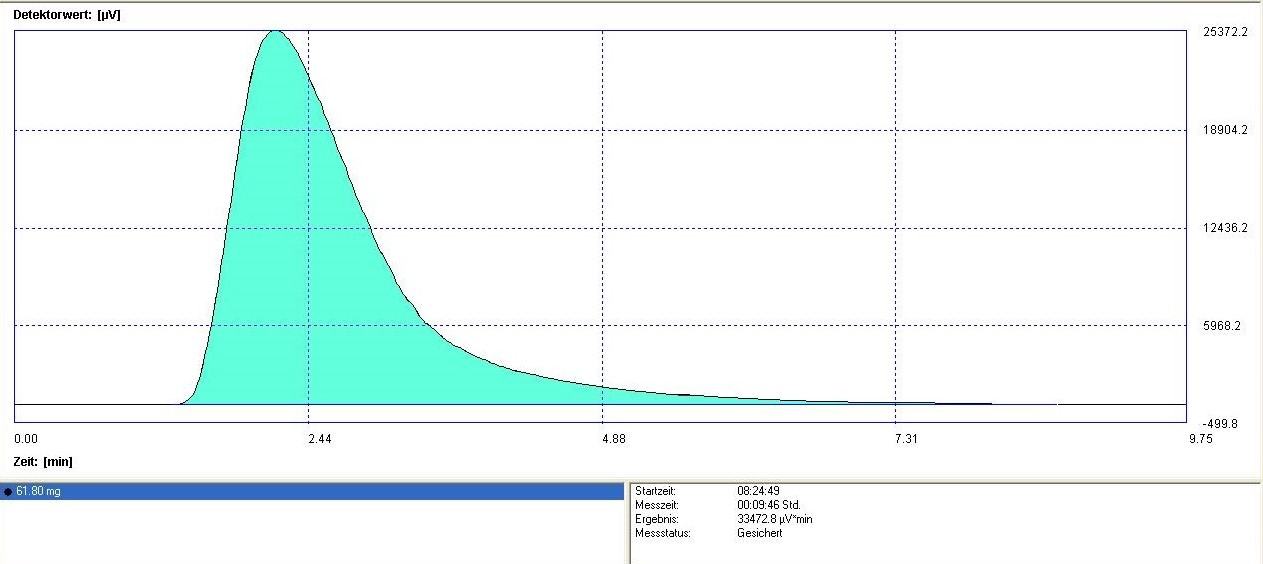
\includegraphics[width=0.75\textwidth]{img/CaCO3_k1}
	\caption{Messkurve 1 für Kalibrierung mit \ce{CaCO3}}
	\label{dia:k1}
\end{figure}
\FloatBarrier
%Ende

%Start
\begin{figure}[h!]
	\centering
	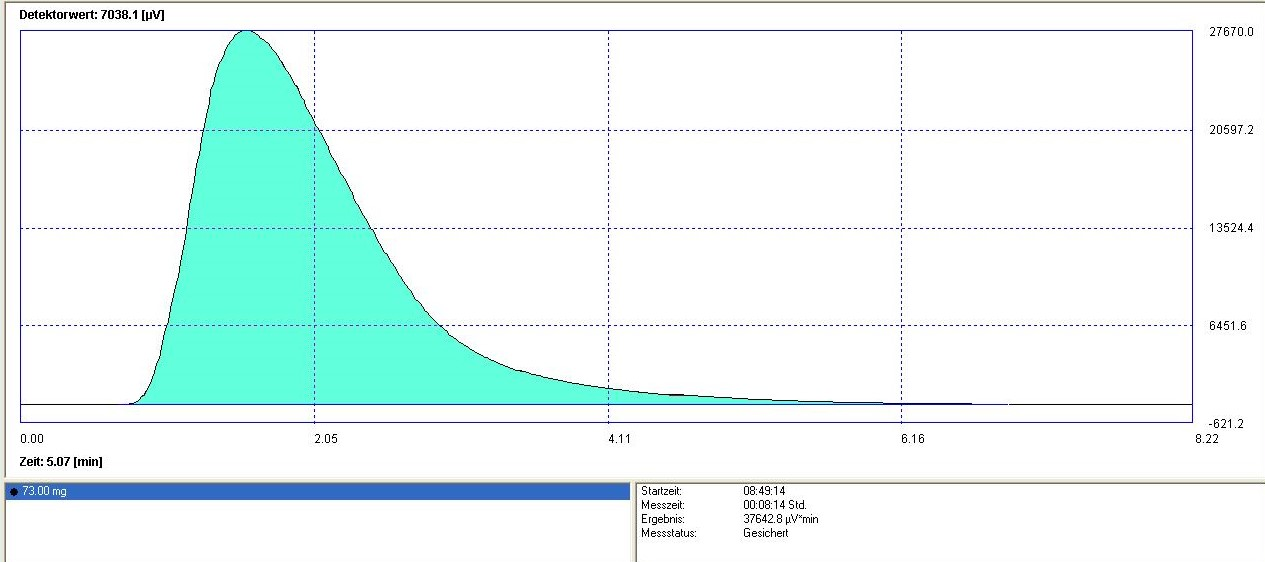
\includegraphics[width=0.75\textwidth]{img/CaCO3_k2}
	\caption{Messkurve 2 für Kalibrierung mit \ce{CaCO3}}
	\label{dia:k2}
\end{figure}
\FloatBarrier
%Ende

%Start
\begin{figure}[h!]
	\centering
	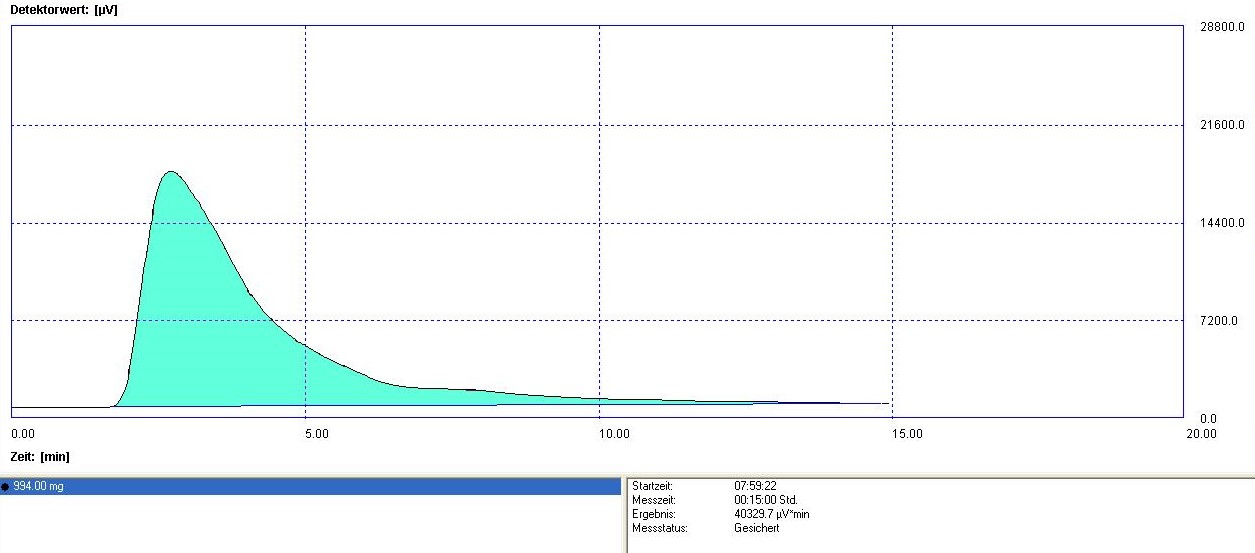
\includegraphics[width=0.75\textwidth]{img/Muell_V1}
	\caption{Messkurve für Müllprobe 1}
	\label{dia:m1}
\end{figure}
\FloatBarrier
%Ende

%Start
\begin{figure}[h!]
	\centering
	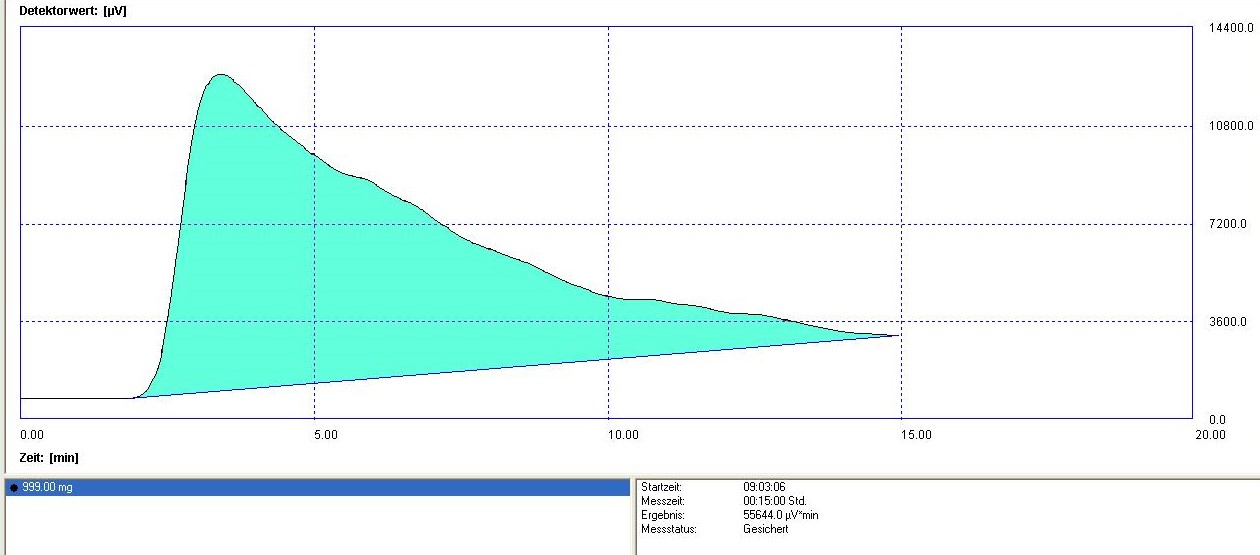
\includegraphics[width=0.72\textwidth]{img/Muell_V2}
	\caption{Messkurve für Müllprobe 2}
	\label{dia:m2}
\end{figure}
\FloatBarrier
%Ende

\newpage

Um die Messwerte im Vergleich zu den Blindproben beurteilen zu können sind diese im Diagramm \ref{dia:kalibrierkurve} aufgezeigt und werden mittels Abweichungsrechnung ab Gleichung \ref{gl:abweichung} weiter analysiert.

\begin{figure}[h!]
	\begin{center}
		\begin{tikzpicture}
		\begin{axis}[
		xlabel={$m_{Carbonat} \left[\si{\milli \gram}\right]$},
		ylabel={$\Phi \left[\si{\micro \volt \minute}\right]$},
		xmin = 0,
		xmax = 120,
		width= 15cm,
		height=6cm,
		ymin=0,
		ymax=70000,
		axis x line=bottom,
		axis y line=left,
		legend style={
			at={(0.2,-0.25)},anchor=north west}]
		
		\addplot [domain=0:200, samples=101,dotted]{540.24*x + 54.501};
		\addlegendentry{Verlauf der Messdaten $(540,24*x + 54,50)$};
		%\addplot [domain=0:200, samples=101,dashed]{476.91*x + 3876.1};
		\addplot [domain=0:200, samples=101,]{524.41*x + 141.53};
		\addlegendentry{Kalibrierkurve $(524,41*x + 141,53)$};
		\addplot+ [mark=*, color=black] coordinates {(74.55,40329.7)};
		\addlegendentry{\ce{CaCO3}-Müllprobe 1};
		\addplot [mark=*, color=black] coordinates {(102.9,55644.0)};
		\addlegendentry{\ce{CaCO3}-Müllprobe 2};
		\addplot [mark=x, color=blue, only marks] coordinates {(61.8,33472.8) (73.0,37642.8) (0,0)};
		\addlegendentry{\ce{CaCO3}-Blindproben};
		
		\addplot [mark=x, color=red] coordinates {(74.5,40329.7)};
		\addlegendentry{Kalibrierpunkt (berechnet)};
		\end{axis}%
		\end{tikzpicture}%
	\end{center}
	\caption{Kalibrierkurve zur Bestimmung des Carbonatgehaltes der  Müllprobe II}
	\label{dia:kalibrierkurve}
\end{figure}
\FloatBarrier
\vspace*{-7mm}
\subsubsection{Abweichung von Kalibrierkurve}
\vspace*{-3mm}
\begin{flalign}
\label{gl:abweichung}
	a	&= \frac{\Phi_{Mess}-\Phi_{Kali}}{\Phi_{Kali}}\\[2mm]
	a_1	&= \frac{\SI{40329.7}{\micro \volt \minute}-\SI{39236,30
		}{\micro \volt \minute}}{\SI{39236,30
	}{\micro \volt \minute}} = \underline{\underline{2,8\%}}\\[2mm]
	a_2	&= \frac{\SI{55644.0}{\micro \volt \minute}-\SI{54101,75}{\micro \volt \minute}}{\SI{54101,75
		}{\micro \volt \minute}} = \underline{\underline{2,9\%}}
\end{flalign}

\newpage

\subsection{Bestimmung des TC}
\label{sec:tc}
\textcolor{red}{Bisschen Text und Verweis auf Durchführung wären schön}\\
Analog dazu ergab die direkte Messung mittels \textit{Analysegerät} einen Wert von \SI{274,26}{\gram \per \kg} für den $TC$ der originalen Müllprobe II.

\begin{figure}[h!]
	\renewcommand{\arraystretch}{1.2}
	\centering
	\caption{TC der Blindprobe, der originalen und der vorbehandelten Abfallprobe}
	\label{tab:tc_messung}
	\begin{tabular}{c|c|c}
		\hline
		\textbf{Probe} & \textbf{Probenmenge} & \textbf{Messwert}  \\
		\hline
		Blindprobe				&	\SI{234,3}{\milli \gram}	& \SI{0,41}{\mpercent}	\\
		Original				&	\SI{79,0}{\milli \gram}	& \SI{27,43}{\mpercent}		 \\
		Vorbehandelt mit TIC	&	\SI{474,9}{\milli \gram}	& \SI{4,39}{\mpercent}\\
		\hline
	\end{tabular}
\end{figure}
\FloatBarrier

\subsection{Bestimmung des TOC}
\textcolor{red}{ÜBERARBEITEN MIT TOC BERECHNUNG}
\begin{flalign}
	TOC	&= TC-TIC
\end{flalign}

\begin{figure}[h!]
	\renewcommand{\arraystretch}{1.2}
	\centering
	\caption{Daten zu den Kohlenstoffgehalten der originalen Abfallprobe II}
	\label{tab:kohlenstoffgehalte}
	\begin{tabular}{c|c|c||c}
		\hline
		\textbf{Kohlenstofftyp} & \textbf{Messwert} & \textbf{Berechnet} & \textbf{Mittelwert}  \\
		\hline
		TC		&	\SI{27,43}{\mpercent}	& -							& $\approx \SI{27}{\mpercent}$ \\
		TIC		&	\SI{1,1}{\mpercent}		& -							& $\approx \SI{1}{\mpercent}$ \\
		TOC		&	-						& \SI{26,33}{\mpercent}		& $\approx \SI{26}{\mpercent}$\\
		\hline
	\end{tabular}
\end{figure}
\FloatBarrier

\newpage

\section{Bestimmung von Brenn- und Heizwert}
In diesem Abschnitt werden die Berechnungen und Ergebnisse zur Bestimmung der Trockensubstanz $TS$, des Wassergehaltes $W$, sowie des Glühverlustes $GV$ dargestellt. \\
Brenn- und Heizwert wurden mittels Näherungsformeln nach \textsc{Shin} bestimmt und geben Auskunft über die Wertigkeit der Müllprobe als Ersatzbrennstoff. Für die Berechnung wurden die Ergebnisse aus Tabelle \ref{tab:ts_w_gv} genutzt.

\subsubsection{Bestimmung des Trockensubstanzgehalt $\mathbf{TS}$} 
\begin{flalign}
TS \left[\%\right]	&= \frac{m_{\text{Trockensubstanz}}}{m_\text{gesamt}}*100\%\\
TS_{\text{TIC}}		&= \frac{\SI{7,340}{\gram}}{\SI{38,717}{\gram}}*100\%\\
&=\underline{18,96\%}\\[2mm]
TS_{\text{org.}}		&= \frac{\SI{2,878}{\gram}}{\SI{2,976}{\gram}}*100\%\\
&=\underline{96,71\%}
\end{flalign}

\subsubsection{Bestimmung des Wassergehaltes $\mathbf{W}$} 
%Trockensubstanz TIC = 38,717 dann 7,340
%TS original = 2,976 dann 2,878
\begin{flalign}
W \left[\%\right]	&= \frac{m_\text{gesamt}-m_{\text{Trockensubstanz}}}{m_\text{gesamt}}*100\%\\
W_{\text{TIC}}		&= \frac{\SI{38,717}{\gram}-\SI{7,340}{\gram}}{\SI{38,717}{\gram}}*100\%\\
&=\underline{81,04\%}\\[2mm]
W_{\text{org.}}		&= \frac{\SI{2,976}{\gram}-\SI{2,878}{\gram}}{\SI{2,976}{\gram}}*100\%\\
&=\underline{3,29\%}
\end{flalign}

\subsubsection{Bestimmung des Glühverlustes $\mathbf{GV}$}
%VERBENNUNG
\begin{flalign}
GV \left[\%\right]				&= \frac{m_{\text{gesamt}}-m_{\text{Glührückstand}}}{m_\text{gesamt}}*100\%\\[2mm]
GV_{\text{org.}} &= \frac{\SI{2,878}{\gram}-\SI{2,203}{\gram} }{\SI{2,878}{\gram}}*100\%\\
&= \underline{\SI{23,45}{\percent}}
\end{flalign}

\subsubsection{Bestimmung des Inertstoffgehaltes $\boldsymbol{IS}$}
%VERBENNUNG
\begin{flalign}
IS\left[\%\right]				&= \SI{100}{\percent}-TC-W\\
IS_{\text{org.}} &\approx \SI{100}{\percent}-\SI{25}{\percent}-\SI{3}{\percent}\\
&\approx \underline{\SI{72}{\percent}}
\end{flalign}

%Tabelle START
\vspace*{-.5cm}
\renewcommand{\arraystretch}{1.2}
\begin{table}[h!]
	\centering
	\caption{Daten zu Trockensubstanz, Wassergehalt, Glühverlust und \mbox{Inertstoffgehalt} \\ der Müllprobe 2}
	\label{tab:ts_w_gv}
	%\resizebox{10cm}{!}{
	\begin{tabulary}{1.2\textwidth}{C|CC|CC}
		\hline
		\textbf{Probe} & \textbf{Trockensubstanz} & \textbf{Wassergehalt} & \textbf{Glühverlust} & \textbf{Inertstoffgehalt}\\ 
		\hline
		Original & 96,71\% & 3,29\% & 23,45\%&76,55\%\\
		Nach TIC & 18,96\% & 81,04\% & - & -\\
		\hline
	\end{tabulary}
	%}
\end{table}
\FloatBarrier
\vspace*{-2.5mm}
%Tabelle Ende

\subsubsection{Bestimmung des Brennwertes $\mathbf{H_s}$}
\begin{flalign}
	H_s \left[\si{\kilo \joule \per \kg}\right]		&= 523*GV^{0,77}\\
	H_s(org.)	&= 523*23,45^{0,77}\\	
				&= \underline{\underline{\SI{5936,24}{\kilo \joule \per \kg}\approx\SI{5,94}{\mega \joule \per \kg}\approx\SI{1,65}{\kWh \per \kg}}}
\end{flalign}


\subsubsection{Bestimmung des Heizwertes $\mathbf{H_i}$} 
\begin{flalign}
H_i	\left[\si{\kilo \joule \per \kg}\right]	&= H_s*\frac{TS}{100}-25*\left(0,09*H*TS+W\right)\\
											&= H_s*\frac{TS}{100}-25*\left(0,09*\frac{GV}{15}*TS+W\right)\\[2mm]
H_i(org.)		&= \SI{5936,24}{\kilo \joule \per \kg}*\frac{96,71}{100}-25*\left(0,09*\frac{23,45}{15}*96,71+3,29\right)\\
				&= \underline{\underline{\SI{5318,51}{\kilo \joule \per \kg}\approx\SI{5,32}{\mega \joule \per \kg}\approx\SI{1.48}{\kWh \per \kg}}}
\end{flalign}
 


\chapter{Diskussion}
\label{sec:diskussion}

Plausibilität Heizwert

Plausibilität Brennwert

Plausibilität TS

Plausibilität Wassergehalt

Plausibilität Glühverlust

Plausibilität Carbonatgehalt

Plausibilität TIC


Die wichtigste anorganische Kohlenstoffquelle in der Müllprobe sind vermutlich Carbonate.
Carbonate sind wichtige Füll- und Zuschlagsstoffe für Papier, Pappe und diverse Kunststoffe. Herkömmliches Papier kann dabei einen Füllstoffanteil von bis zu 30 \% aufweisen. In Kunststoffen dient Calciumcarbonat unter anderem zur Steigerung der Schlagfestigkeit. 

Die unbekannte Zusammensetzung der Müllprobe und die uneinheitliche Anwendung von Zuschlag- und Füllstoffen lassen kaum einen Vergleich mit anderen Proben zu. 



Wikipedia::
Wichtige Füllstoffe von thermoplastischen Kunststoffen sind:

Glasfasern, Glaskugeln und Glasbruch
mineralische Füllstoffe wie Calciumcarbonat und Talkum
Kohlenstofffasern (Kurzfasern)
Ruße

Bei der Papierherstellung werden vor allem Silikate, meist Kaolin, eine weiße Porzellanerde, als Füllstoff verwendet. Kaolin macht das Papier undurchsichtiger (opaker), weißer und erhöht die Rohdichte. Auch gibt der Füllstoff dem Papier eine glattere Oberfläche, da er die Hohlräume zwischen den Fasern auffüllt. Papier kann, abhängig von der Sorte, bis zu 30 % Füllstoff enthalten.

Als Füllstoff werden oft Carbonate verwendet, meistens Kreide, aber ebenso Sulfate wie Gips oder Oxide, beispielsweise Titandioxid. Bariumsulfat kommt als Füllstoff zur Herstellung von Barytpapier in Betracht, das dadurch auffallend schwer ist.[3] 

Heizwerte Plausibel siehe Quelle\\

In der Endkonsequenz könnte jeder Carbonatgehalt durch Füllstoffe erklärt werden. Ein weiterer Einflussfaktor sind Verunreinigungen. Teilweise werden anfallende Abfälle nicht korrekt getrennt. Ein wahrscheinliches Szenario wäre die Entsorgung nicht vollkommen restentleerter Kalksäcke. Die Säcke bestehen aus einer Kunststoffschicht und einer äußeren Papierhülle. Der enthaltene Kalk verfälscht die Messergebnisse. Ebenso könnte Kehricht im untersuchten Müll entsorgt worden sein.


Quelle in der Bibliothek suchen

Plausibilität TC

Plausibilität Cl-Gehalt\\

%\begin{tikzpicture}
%\begin{axis}[
%xbar=1pt,% space of 0pt between adjacent bars
%bar width=11,
%width=15cm,
%height=11cm,
%%minor y tick num=4,
%xmax=40,xmin=-40,
%x tick label style={/pgf/number format/.cd,%
%	scaled x ticks = false,
%	set decimal separator={,},
%	fixed},
%symbolic y coords={Zn,Cl,Mn,Uub,As},
%ytick=data,
%xtick={-30.5,-20.5,-10.5,0,10.5,20.5,30.5},
%grid=major,
%%enlargelimits=0.15,
%]
%\addplot coordinates {
%	(-10.3,Mn) (15.4,Cl) (5,Zn) (24,Uub) (30,As)
%};
%\addplot coordinates {
%	(-3,Mn) (5,Cl) (15,Zn) (20,Uub) (35,As)
%};
%\addplot coordinates {
%	(-8,Mn) (-19,Cl) (20,Zn) (30,Uub) (5,As)
%};
%
%\end{axis}
%\end{tikzpicture}

\nocite{ersatzbrennstoffe,PolymerServiceGmbHMerseburg.13.08.2019,Wikipedia.21.11.2019,Skript}

\chapter{Fehlerbetrachtung}
\label{sec:fehler}

Es ist zu bezweifeln, dass alle im Müll enthaltenen Carbonate mit der Phosphorsäure reagieren konnten. Papier ist sehr porös und saugt sich mit der sauren Lösung voll. Die Füllstoffpartikel liegen zwischen den Fasern vor und können so bis auf wenige Ausnahmen von der Phosphorsäure erreicht werden. Probleme treten auf wenn polymerbeschichtete Zelluloseerzeugnisse oder Kunststoffe zu analysieren sind. Die Carbonate in der aller äußersten Schicht können reagieren, während alle restlichen Carbonatpartikel von der Kunststoffmatrix umhüllt und damit von der umgebenden Lösung getrennt sind. Um auch diese Anteile erreichen zu können müsste der Müll kleinstmöglich zerkleinert werden. Thermoplastische Kunststoffe und Elastomere können nur mit großem Aufwand so klein zerteilt werden. Ihr (visko-)elastisches Verhalten stellt dabei die größte Herausforderung dar. Sie können dadurch nur geschnitten, gerissen oder geschert werden. Mühlen die das Mahlgut auf Druck belasten oder die Teilchen durch Impulse und Prall brechen sind nicht geeignet.
Alternativ zum Mahlen ließe sich vielleicht eine Veraschung bewerkstelligen, bei der die Carbonate keinen Temperaturen ausgesetzt sind, bei denen sie dissoziieren. Die Asche enthielte dann den gesamten anorganischen Kohlenstoff in leicht zu analysierender Form.\\

Der Stoffumsatz im Reaktor muss als nicht vollständig angenommen werden da die Messung aus Zeitgründen gestoppt wurden, als der gemessene emittierte Kohlenstoffdioxidstrom noch nicht null war. Obige Einschlüsse in inerte Matrizen begünstigen ebenso die Unvollständigkeit der Reaktion. Für eine allgemeine Einschätzung der Müllprobe scheint dieses Vorgehen jedoch als ausreichend.\\
Der Detektor unterliegt zufälligen Messabweichungen. Eine Fehlerklasse zum verwendeten Gerät ist nicht bekannt.\\

Betrachtet man die Partikelgröße, innerhalb der Müllprobe, schwankte diese stark. Es war von Fasern mit vielleicht \SI{5}{\milli\meter} bis zu Staub mit etwa \SI{100}{\micro\meter} alles vorhanden. Viel bedeutender ist das Verhältnis der enthaltenen Kunststoffe, dem Papier, der Pappe und den Inertstoffen untereinander. Schon das Vorhandensein eines Polyvinylchloridpartikels kann den ermittelten Chlorgehalt stark vom wahren mittleren Chlorgehalt abweichen lassen. Ähnlich verhält es sich auch für Schwefel- und Kohlenstoffgehalte.\\

Das zugegebene destillierte Wasser könnte durch Spuren von Kalk verunreinigt gewesen sein. Die eventuell enthaltenen Carbonate hätten dann den Messwert nach oben verschoben.\\

Die Dichtigkeit des Apparates könnte Mangelhaft gewesen sein. Das Vermögen des Behälters einen bestimmten Gasdruck über einen längeren Zeitraum zu halten wurde nicht geprüft. Jedoch wäre ein großes Leck aufgefallen und wurde demnach nicht registriert. Kleine Verluste sind allerdings nicht auszuschließen und hätten den bestimmten Carbonatgehalt gesenkt.\\

Geht man weiter auf die Messergebnisse und deren Auswertung ein, so ist gerade bei der Bestimmung des Carbonatgehaltes eine exaktere Kalibrierung durch weitere Blindproben notwendig um eine genauere Kalibrierkurve zu erhalten. Gerade die Abweichungen von $\approx \SI{3}{\percent}$ können maximal als grobe Einschätzung gewertet werden und entsprechen keiner Laborqualität. Die Qualität der Blindprobe ist bestenfalls ausreichend. Versuchsbetreuer bestätigten, dass es sich um eine ältere Chemikalie handelt welche bereits über lange Zeit Luftfeuchtigkeit und Kohlenstoffdioxid ausgesetzt war. \linebreak

Da während der Bestimmung des TIC die erste Müllprobe verloren ging, wurde eine zweite Müllprobe im weiteren Verlauf des Versuches analysiert. Dies zeigt sich unter Abschnitt \ref{sec:tic}. Die anschließend analysierte Probe wurde der ursprünglichen jedoch genauest-möglich nachempfunden. Eine nahezu ähnliche Menge Abfall des Mülls II wurde mit der exakt gleichen Menge Phosphorsäure versetzt und anschließend getrocknet.\linebreak

Optisch ließen sich jedoch Unterschiede in der Zusammensetzung erkennen. So erhielt die erste Probe der Müllprobe II mehr Textilfaser und die zweite Probe der Müllprobe II mehr Papier, Pappe und vermutlich auch Kunststoffstückchen.\linebreak
Das könnte ein Grund für den \SI{3}{\percent} höheren Carbonatgehalt, der zweiten Probe sein, da gerade in Papier, Pappe und Kunststoffen oft auch Carbonate als Füllstoffe zugesetzt werden. So finden sich in Papier, je nach Sorte, bis zu \SI{30}{\mpercent} Füllstoffe wie Kaolin, Kreide (Carbonate) oder Gips \cite{Wikipedia.21.11.2019} und in Kunststoffen bis zu  \SI{40}{\mpercent} Carbonate wieder \cite{PolymerServiceGmbHMerseburg.13.08.2019}, um den geforderten Eigenschaften gerecht zu werden.\\
Zu den berechneten Heiz- und Brennwerten ist noch zu erwähnen, dass diese nur mittels Näherungsformeln berechnet wurden und somit nur eine grobe Einschätzung zulassen. Jedoch ist eine genauere Berechnung für diesen Versuch nicht nötig gewesen, da der Charakter der Müllprobe II deutlich wurde und durch Inhomogenität des Mülls eine größere Genauigkeit der Heiz- bzw. Brennwertbestimmung keinen Mehrwert für diesen Versuch gibt.\\ \\

Bei der Bestimmung des Aschegehaltes vielen 5 Fehlerquellen auf. Der Müll könnte durch einen beachtlichen mineralischen Feststoffanteil belastet sein. Die Veraschung könnte unvollständig sein, wodurch verbliebene Organische Anteile als anorganisch interpretiert würden. Die Asche könnte bei den angewendeten Temperaturen ihre chemische Zusammensetzung in Anwesenheit von Umgebungsluft verändert haben. Die Asche könnte Feuchtigkeit aus der Umgebungsluft aufgrund ihrer hygroskopischen Eigenschaften angezogen haben. Es könnten abermals Messfehler passiert sein. 

\chapter{Fazit}
Abschließend lässt sich sagen, dass die Charakterisierung der Müllprobe II mit den dargelegten Messmethoden für eine grobe, qualitative Einschätzung des Mülls geeignet ist. Genauere Messmethoden könnten bei tieferer Charakterisierung nötig sein, gerade wenn es um die quantitative Zusammensetzung des Mülls geht.

\textbf{wie wärs damit?}

Abschließend lässt sich sagen, dass die in diesem Versuch angewendete Methodik zur groben Einordnung der Müllprobe ausreicht. Eine belastbare qualitative und quantitative Analyse würde weitere Messungen mit verbesserter Technik erfordern.

%Praktikumsskript, Modul ………, Versuch …….., Prof. Musterprof. 
%DIN 12345, Jahr der Veröffentlichung 
%Link der Internetseite, Zugriffsdatum 
%Buchtitel, Autor, Verlag, Veröffentlichungsjahr 
\nocite{*}

%Literaturverzeichnis Bücher
\bibliography{Literatur}
\bibliographystyle{unsrtdin}
\addcontentsline{toc}{chapter}{Literaturverzeichnis}







%Anhang
\addcontentsline{toc}{chapter}{Anhang}

%\chapter*{Eidesstattliche Erklärung}
\label{erklaerung}
Hiermit versichere ich, die vorliegende Seminararbeit selbstständig und nur unter Verwendung der von mir angegebenen Quellen und Hilfsmittel verfasst zu haben. Sowohl inhaltlich als auch wörtlich entnommene Inhalte wurden als solche kenntlich gemacht. Die Arbeit hat in dieser oder vergleichbarer Form noch keinem anderem Prüfungsgremium vorgelegen. \\
\\[1.5cm]
Datum:	\hrulefill\enspace Unterschrift: \hrulefill
\\[3.5cm]
\addcontentsline{toc}{chapter}{Selbstständigkeitserklärung}

%\chapter{Bausteine}

\section{Beispiel für Tabelle}

%Tabelle START
\vspace*{-2.5mm}
\renewcommand{\arraystretch}{1.2}
\begin{table}[h!]
	\centering
	\caption{Abmessungen der Probekörper vor dem Zugversuch}
	\label{tab:tabelle1}
	%\resizebox{10cm}{!}{
	\begin{tabulary}{\textwidth}{C|CCC}
		\hline
		\textbf{Probe}  &\textbf{Breite [mm]}&\textbf{Dicke [mm]}&\textbf{Anf.-länge[mm]} \\ 
		\hline
		Kupfer (gewalzt) & 12,5 &3,00&50\\
		Kupfer (geglüht) & 12,5&3,00&50\\
		PA6 & 10,0&4,00&50\\
		PP (EPR-30\% Kautschuk) & 9,9 &3,95&50\\
		\hline
	\end{tabulary}
	%}
\end{table}

\FloatBarrier
\vspace*{-2.5mm}
%Tabelle ENDE

\section*{Tabelle mit Itemize}
%Tabelle START
\vspace*{-2.5mm}
\renewcommand{\arraystretch}{1.2}
\begin{table}[h!]
	\centering
	\caption*{Vor- und Nachteile der Geothermie}
	\label{tab:tabelle1}
	\begin{tabulary}{\textwidth}{C|C}
		\hline
		\textbf{Vorteile}  &\textbf{Nachteile} \\ 
		\hline
		&\\
		\begin{minipage}[t]{0.4\textwidth}
			\begin{itemize}
				\item Strom, Wärme und Kälte wird erzeugt
				\item keine saisonalen und tageszeitlichen Schwankungen
				\item 	quasi-regenerativ
				\item 	nachfrage-gerechte Energiebereitstellung
				\item Erzeugungspotenzial sehr hoch 
				\item 	grundsätzlich standortunabhängig
			\end{itemize}
		\end{minipage} & 
		\begin{minipage}[t]{0.4\textwidth}
			\begin{itemize}
				\item hohe Anschaffungskosten
				\item abhängig von geologischen Gegebenheiten
				\item geringer Stromwirkungsgrad (thermodynamisch bedingt)
				\item keine Marktdurchdringung in DE
				\item erfahrene Bauunternehmen notwendig
				\item gute Vorerkundung und Überwachung notwendig
			\end{itemize}
		\end{minipage}\\
	\end{tabulary}
\end{table}
\FloatBarrier
\vspace*{-2.5mm}
%Tabelle ENDE

\newpage

\section*{Beispiel für Skalierbare Tabelle}
%TAbelle Start
\vspace*{-2.5mm}
\renewcommand{\arraystretch}{1.2}
\begin{table}[h!]
	\centering
	\caption*{}
	\resizebox{0.5\textwidth}{!}{
		\begin{tabulary}{\textwidth}{C|C|C|C}
			\textbf{Name} & \textbf{Anwendung}&\textbf{Gleichung}&\textbf{Stoffkonstante} \\ 
			\hline  
			KICK& $x_{80_\omega}>\SI{50}{\milli\meter}$ &$e_{KICK}=c_K*log(\frac{x_{80_\omega}}{x_{80_\alpha}})$&$c_K=1,15*\frac{c_B}{\sqrt{0,05\si{\meter}}} \left[\si{\raiseto{2}\meter\per\raiseto{2}\second}\right]$\\
			BOND&$\SI{50}{\micro\meter}<x_{80_\omega}<\SI{50}{\milli\meter}$&$e_{BOND}=c_B*\left(\frac{1}{\sqrt{x_{80_\omega}}}-\frac{1}{\sqrt{x_{80_\alpha}}}\right)$& $c_B$: tabelliert $\left[\si{\raiseto{2,5}\meter\per\raiseto{2}\second}\right]$\\ 
			RITTER& $x_{80_\omega}>\SI{50}{\micro\meter}$&$e_{RITT}=c_R*\left(\frac{1}{x_{80_\omega}}-\frac{1}{x_{80_\alpha}}\right)$&$c_R= 0,5*c_B*\sqrt{\SI{5e-5}{\meter}}$ \\  
	\end{tabulary}}
\end{table}
\FloatBarrier
%Ende TAbelle

\section{Befehlszeilen in Text einfügen}
Befehlzeilen aus der "Latex-Sprache"\ lassen sich nicht ohne weiteres im Text darstellen. Das System erkennt diese als solche und gibt warnhinweise aus. In der Regel werden die Befehle dann auch falsch dargestellt. Umgehen lässt sich diese Problematik mit der verbatim-Umgebung. In ihren Grenzen werden Eingaben 1:1 dargestellt wie eingegeben. Die Funktionsweise soll nachfolgend durch ein Beispiel verdeutlicht werden.
\begin{verbatim*}

\begin{verbatim}
\usepackage{Beispieltrolllllollllolll} 
\end{verbatim}

\end{verbatim*}

Sollte besonderer Wert auf die Kenntlichmachung der Leerzeichen gelegt werden kann auch mit \texttt{verbatim*} gearbeitet werden.

\section{Seitenübergreifende, lange Tabellen}

Tabellen welche Messwerte in einem solchen Umfang enthalten, dass sie nicht auf einer einzelnen A4-Seite Platz finden, können mit dem Paket \begin{verbatim}
\usepackage{longtable} 
\end{verbatim}
in ein Dokument eingepflegt werden wie folgendes Beispiel belegt.:
\begin{longtable}[c]{lllll}
	\caption{Dehnungstabelle}\\
	\label{alles}
	$Zeit [HH:MM:SS]$ & $\Delta l_{PE} [mm]$ & $\varepsilon_{PE}$ & $\Delta l_{Pb} [mm]$ & $\varepsilon_{Pb}$ \\
	\hline
	\endfirsthead
	%\caption{}\\
	$Zeit [HH:MM:SS]$ & $\Delta l_{PE} [mm]$ & $\varepsilon_{PE}$ & $\Delta l_{Pb} [mm]$ & $\varepsilon_{Pb}$ \\ 
	\hline
	\endhead
	\multicolumn{5}{r}{Fortsetzung auf n{\"a}chster Seite}\\
	\endfoot
	\hline
	\multicolumn{5}{r}{} \\
	\endlastfoot
	% Ab hier kommt der Inhalt der Tabelle
	00:00:00 & 3,00 & 0,11 & 3,30 & 0,12\\
	00:00:10 & 3,80 & 0,14 & 3,42 & 0,13\\
	00:00:20 & 4,15 & 0,16 & 3,53 & 0,13\\
	00:00:30 & 4,43 & 0,17 & 3,68 & 0,14\\
	00:00:40 & 4,61 & 0,17 & 3,71 & 0,14\\
	00:00:50 & 4,80 & 0,18 & 3,81 & 0,14\\
	00:01:00 & 4,95 & 0,19 & 4,12 & 0,15\\
	00:20:00 & 8,03 & 0,30 &  & \\
\end{longtable} 

\section{Diagramme}
Diagramme lassen sich unter anderem mit dem Paket 
\begin{verbatim}
\usepackage{pgfplots} 
\end{verbatim}
implementieren.
Um das Dokument einigermaßen klein zu halten empfehle ich folgendes weiters Paket zu nutzen.
\begin{verbatim}
\usepackage{csvsimple} 
\end{verbatim}
Es erleichter das importieren von Datensätzen aus .csv Dateien. Die .csv Datei muss folgenden Anforderungen genügen:- Dezimaltrenner Punkt
\begin{itemize}
	\item Dezimaltrenner Punkt
	\item Jede Zeile umgebrochen
	\item Koordinaten durch komma getrennt
	\item Spalten beschriften z.B x,y oder a,b
\end{itemize}

Sollte man eine Tabellenkalkulationsdatei in eine csv Datei konvertiert haben, hat dieses meist die Falsche Form. Durch die Funktion suchen und ersetzen (bsp emacs) können aber sehr schnell die nötigen Korrekturen erfolgen. 

\begin{figure}[h]
	\begin{center}
		\begin{tikzpicture}
		\begin{axis}[
		width=12cm,
		height=6cm,
		xlabel=Zeit in Sekunden,
		ylabel=Dehnung]
		
		\begin{scope}[brown]
		\draw[brown] ({axis cs:10,0}|-{rel axis cs:0,1}) -- ({axis cs:10,0}|-{rel axis cs:0,0});
		\draw[brown] ({axis cs:120,0}|-{rel axis cs:0,1}) -- ({axis cs:120,0}|-{rel axis cs:0,0});
		\end{scope} 
		
		\addplot table [x=a, y=b, col sep=comma] {data/KriechkurvePb.csv};
		\end{axis}
		\end{tikzpicture}
		\caption{Kriechkurve Blei}
		\label{kkb}
	\end{center}
\end{figure} 
\FloatBarrier                     

\section*{Beispiel für Berechnungen}
Die Berechnung der wahren Spannung $\sigma_{W}$ bei Höchstkraft erfolgt unter der Annahme, dass der Prüfkörperquerschnitt noch 60\% des Ausgangsquerschnitts beträgt. Die Berechnung erfolgt ab Gleichung \ref{ber1}.\\ 

%Berechnung der Fläche A
\textbf{Fläche} $\boldsymbol{A}$ \textbf{:}
%Start
\begin{flalign}
A 	&= \frac{\pi}{4}*d^2\\
&=\frac{\pi}{4}*(\SI{80}{\milli \meter})^2
\end{flalign}
%Ende

\section{Beispiel für ein Bild}

%Start
\begin{figure}[h!]
	\centering
	\includegraphics[width=0.60\textwidth]{img/skizzepruef3}
	\caption{Skizze Prüfkörperbemaßung}
	\label{skizzepruef}
\end{figure}
\FloatBarrier
%Ende

\newpage

\section{Beispiel für zwei Bilder}
\label{sec:versuchsaufbau}

%Start
\begin{figure}[h!]
	\centering
	\begin{subfigure}{.5\textwidth}
		\centering
		\includegraphics[width=0.75\textwidth]{Aufbau2}
		\caption{Skizze zum Versuchsaufbau}
		\label{fig:sub1}
	\end{subfigure}%
	\begin{subfigure}{.5\textwidth}
		\centering
		\includegraphics[width=0.6\textwidth]{img/Aufbau1}
		\caption{realer Versuchsaufbau}
		\label{fig:sub2}
	\end{subfigure}
	\caption{Versuchsaufbau als Skizze und in Realität}
	\label{fig:aufbau} 
\end{figure}
\FloatBarrier
%Ende

\newpage


\section{Beispiel für vier Bilder}
%Start
\begin{figure}[h!]
	\centering
	\begin{subfigure}{.5\textwidth}
		\centering
		\includegraphics[width=0.75\textwidth]{img/Kupfer_gewalzt}
		\caption{Kupfer (gewalzt)}
		\label{fig:sub3}
	\end{subfigure}%
	\begin{subfigure}{.5\textwidth}
		\centering
		\includegraphics[width=0.75\textwidth]{img/Kupfer_weich}
		\caption{Kupfer (geglüht)}
		\label{fig:sub4}
	\end{subfigure}
	\begin{subfigure}{.5\textwidth}
		\centering
		\includegraphics[width=0.75\textwidth]{img/PA6}
		\caption{PA6}
		\label{fig:sub5}
	\end{subfigure}%
	\begin{subfigure}{.5\textwidth}
		\centering
		\includegraphics[width=0.75\textwidth]{img/PP}
		\caption{PP (ERP-30\% Kautschuk)}
		\label{fig:sub6}
	\end{subfigure}
	
	\caption{Bruchstellennahaufnahmen der Probekörper}
	\label{fig:bruchstellen} 
\end{figure}
\FloatBarrier
%Ende

\section{Beispiel Einheiten}

\begin{align*}
\textbf{$\SI{12,0/12}{\kg\meter\per\second \raiseto{5} \per \xyz}*\SI{13}{\per\raiseto{-2}\meter}=\SI{256}{}$}
\end{align*}

\begin{align}
\SI{12,0/12}{\meter\per\joule}*\SI{13}{\gram}=\SI{256}{\coulomb}
\end{align}

\newpage

\section{Beispiel für Mini-Formelsammlung}
\begin{flalign}
\label{gl1}
\text{\textbf{Dehnung (Def.)} } \boldsymbol{\varepsilon} \text{ \textbf{:}} && \hspace*{-1em}  \varepsilon=\frac{\Delta l}{l_0} &&
\end{flalign}

\begin{flalign}
\label{gl2}
\text{\textbf{norminelle Spannung} } \boldsymbol{\sigma} \text{\textbf{:}} && \hspace*{-3em} \sigma=\frac{F}{A_0} &&
\end{flalign}

\begin{flalign}
\label{gl3}
\text{\textbf{Sekantenmodul (Kunststoffe) }} \boldsymbol{E_S} \text{ \textbf{:}} && E_S=\frac{\sigma_2-\sigma_1}{\varepsilon_2-\varepsilon_1}=\frac{F_2-F_1}{0,002*A_0} &&
\end{flalign}

\begin{flalign}
\label{gl4}
\text{\textbf{E-Modul (Metalle) }} \boldsymbol{E_M} \text{ \textbf{:}} && \hspace*{5em} E_M=\frac{\sigma}{\varepsilon}=\frac{\sigma_2-\sigma_1}{\varepsilon_2-\varepsilon_1}=\frac{R_{p_{0.2\%}}}{0,2\%} &&
\end{flalign}

\begin{flalign}
\label{gl5}
\text{\textbf{Bruchdehnung} } \boldsymbol{A} \text{\textbf{:}} && \hspace*{6em} A= \frac{l_{u}-l_{0}}{l_{0}}*100\% &&
\end{flalign}

\begin{flalign}
\label{gl6}
\text{\textbf{Ausgangsquerschnitt } } \boldsymbol{S_0} \text{\textbf{:}} && \hspace*{3em} S_{0}= Breite*Dicke &&
\end{flalign}
\begin{flalign}
\label{gl7}
\text{\textbf{wahre Spannung} } \boldsymbol{\sigma_{W}} \text{\textbf{:}} &&\hspace*{1em} \sigma_{W}=\frac{F_{max}}{S_{End}}&&
\end{flalign}
\begin{flalign}
\label{gl8}
\text{\textbf{Brucheinschnürung } } \boldsymbol{Z} \text{\textbf{:}} && \hspace*{5em} Z=\frac{S_0-S_u}{S_{o}}*100\% &&
\end{flalign}

\newpage

\section*{Fußnoten}
%Start
\begin{figure}[h!]
	\centering
	\includegraphics[width=0.85\textwidth]{tabdia/kfwerte}
	\caption*{$\text{k}_\text{f}$-Werte der Proben 1 bis 11 \protect\footnotemark[1]}
	\label{}
\end{figure}
\FloatBarrier
%Ende

\footnotetext[1]{bezogen auf $V=\SI{50}{\milli \liter}$ und $h=\SI{10}{\milli \meter}$}



\end{document}
